
\documentclass[a4paper,11pt]{article}

\usepackage{fontspec}
\setmainfont{Calibri}

\linespread{1}

\setlength{\oddsidemargin}{0cm}
\setlength{\evensidemargin}{0cm}
\setlength{\textheight}{23cm}
\setlength{\textwidth}{16cm}

\usepackage{amssymb,mathrsfs,algorithmic,algorithm,multirow}
\usepackage{amsmath,amsbsy,graphicx,color,url,natbib}
\usepackage{ccaption}
\setlength{\bibsep}{0.0pt}

\newcommand{\bm}{\mathbf}
\newcommand{\bs}{\boldsymbol}
\newcommand{\mt}{\mathrm}
\newcommand{\nind}{\noindent}

\usepackage{fancyhdr}
\newcommand{\tstamp}{\today}   
\lhead[\fancyplain{}{\rightmark}]       {\fancyplain{}{}}
\rhead[\fancyplain{}{\rightmark}]       {\fancyplain{}{}}
\chead[\fancyplain{}{\centermark}]       {\fancyplain{}{ENGM214 -- Process Modelling and Simulation} }
\pagestyle{fancyplain}

\usepackage{amsthm}
\theoremstyle{definition}
\newtheorem{exmp}{Example}[section]

\title{\vspace{-2cm} Lecture 2 -- Principles for constructing mechanistic models}

\author{Tao Chen\\
{\small \emph{Department of Chemical \& Process Engineering, University of Surrey, UK}}\\
{\small (email: \texttt{t.chen@surrey.ac.uk}; \hspace{0.5cm} updated on \today )}
}
\date{}

\begin{document}
\maketitle

%\tableofcontents
\vspace{-0.5cm}


\section{The general procedure for building models}

The general procedure is outlined in Fig. \ref{fig:procedure}.
The important considerations have been well covered in the lecture slides.
Here we only stress a few points.

\begin{figure} [!h]
 \begin{center}
	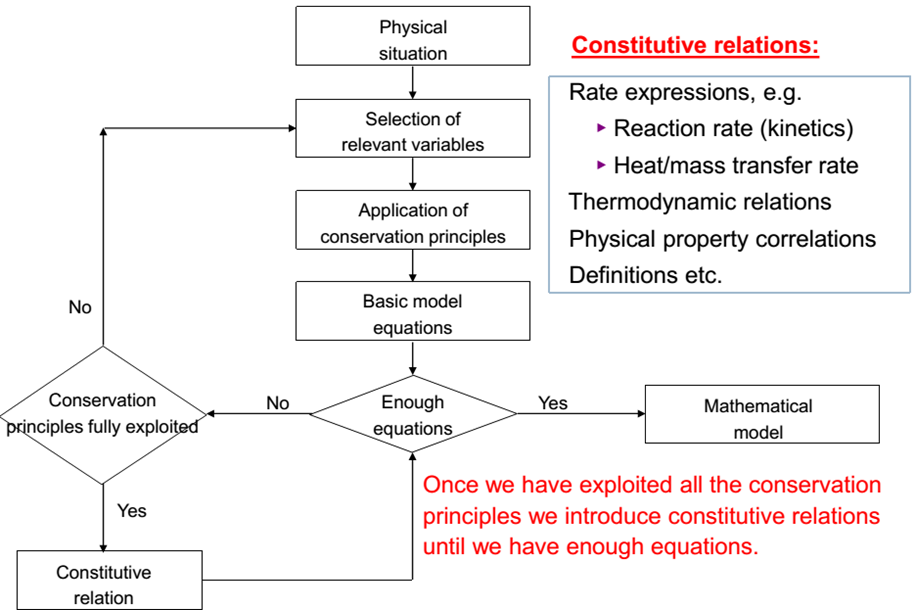
\includegraphics[width=.9\textwidth]{procedure}\\
 \end{center}
 \caption{Overview of the procedure for building models.} 
 \label{fig:procedure}
\end{figure}

\begin{itemize}
	\item \textbf{Modelling has a purpose.} 
\end{itemize}



\section{The concept of degrees of freedom}

\section{A modelling example}


\begin{thebibliography}{2}
\vspace{-0.4cm}
\bibitem[{Hangos(2001)}]{Hangos2001}
	Hangos KM, Cameron IT, 2001. Process Modelling and Model Analysis, Academic Press: London.

\bibitem[{Smith(2004)}]{Smith2004}
	Smith JM, van Ness HC, Abbott MM, 2004. Introduction to Chemical Engineering Thermodynamics, 7th edition, McGraw-Hill.
\end{thebibliography}

\end{document}


